\chapter{Desenvolvimento da EDA}

Nesse capítulo, é aplicado os três passos do ciclo de uma EDA em um contexto prático aplicando o conjunto de dados "Brazilian Cities".

\section{Contextualização}

O IDH (Índice de Desenvolvimento Humano) é um índice que avalia a qualidade de vida em um determinado local, sendo mensurado a partir de 3 fatores: Longevidade, Educação e Renda. No Brasil, o órgão responsável por avaliar o IDH é o IBGE (Instituto Brasileiro de Geografia e Estatística).

Sendo um parâmetro importante, o IDH é capaz de influenciar tomadas de decisões, tais como quais setores aplicar investimento público pelos políticos, se é vantajoso mudar-se para morar nesse local, e se é viável a iniciativa privada investir nesse local para atuar.

Vide na figura \autoref{fig:distribuicao-idh-nas-cidades} a distribuição do IDH nas cidades do Brasil.

\begin{figure}[H]
  \centering
  \caption{\label{fig:distribuicao-idh-nas-cidades}Distribuição do IDH nas cidades brasileiras}
  \label{fig:der}
  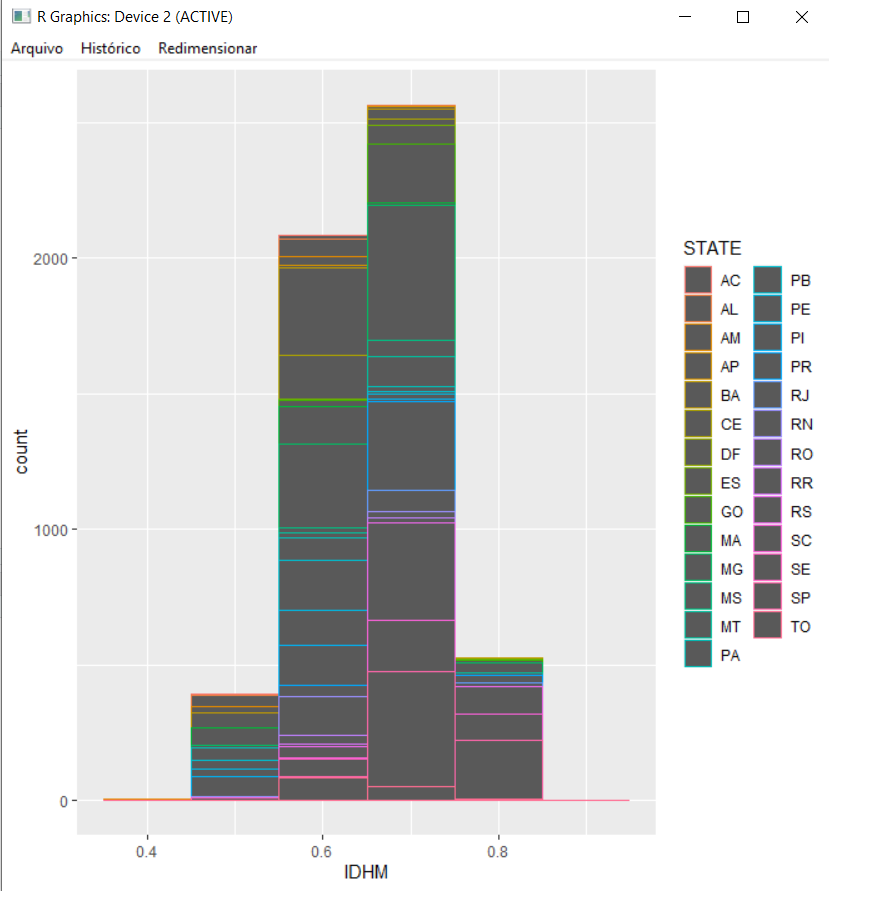
\includegraphics[scale=0.5]{chapter-03-case-01-img-01}
  \legend{Fonte: O autor}
\end{figure}

Visualizando esse gráfico, é perceber que não há cidades brasileiras com IDH menor do que 0.4, nem com IDH maior do que 0.8.

\section{Tratamento de Dados}

Para tornar os dados mais consistentes, foi necessário filtrar os dados cujo IDH não seja NA (Não Aplicável).

\section{Problematização}

Com isso, surgem-se duas questões: 

\begin{enumerate}
	\item "Qual é a razão da discrepância entre os dados de IDH?";
	\item "Por que não existe IDH maior que 1?".
\end{enumerate}

Para responder essas questões, foram feitas análises da variação de cada critério do IDH. Na \autoref{fig:idh-renda}, é analisada a variação de renda. Na \autoref{fig:idh-longevidade}, é analisada a variação de longevidade. E, por fim, na figura \autoref{fig:idh-educacao}, é analisada a variação de educação.

\begin{figure}[H]
  \centering
  \caption{\label{fig:idh-renda}Distribuição do IDH de Renda nas cidades brasileiras}
  \label{fig:der}
  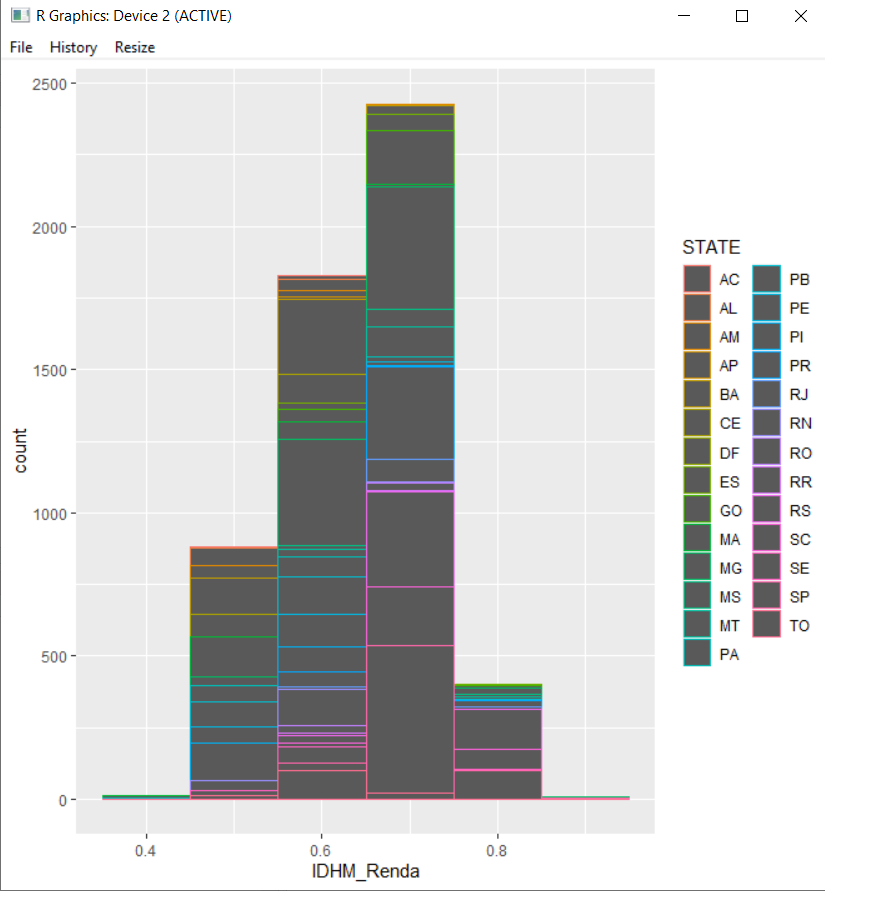
\includegraphics[scale=0.5]{chapter-03-case-01-img-02}
  \legend{Fonte: O autor}
\end{figure}

\begin{figure}[H]
  \centering
  \caption{\label{fig:idh-longevidade}Distribuição do IDH de Longevidade nas cidades brasileiras}
  \label{fig:der}
  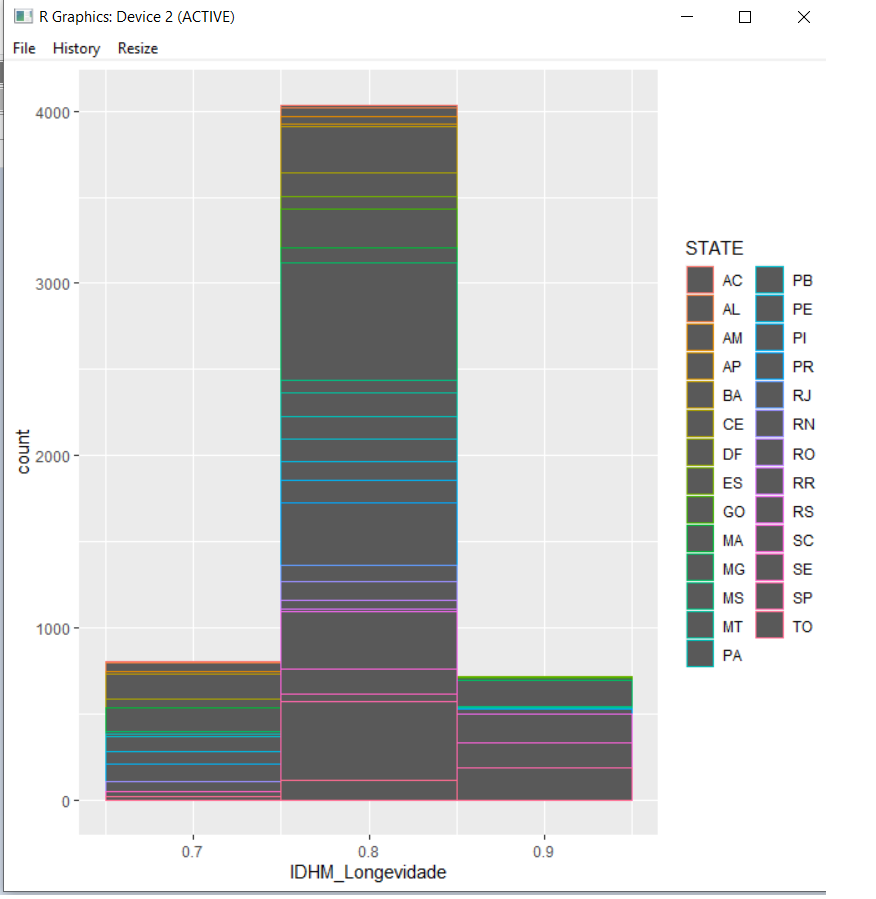
\includegraphics[scale=0.5]{chapter-03-case-01-img-03}
  \legend{Fonte: O autor}
\end{figure}

\begin{figure}[H]
  \centering
  \caption{\label{fig:idh-educacao}Distribuiçãa do IDH de Educação nas cidades brasileiras}
  \label{fig:der}
  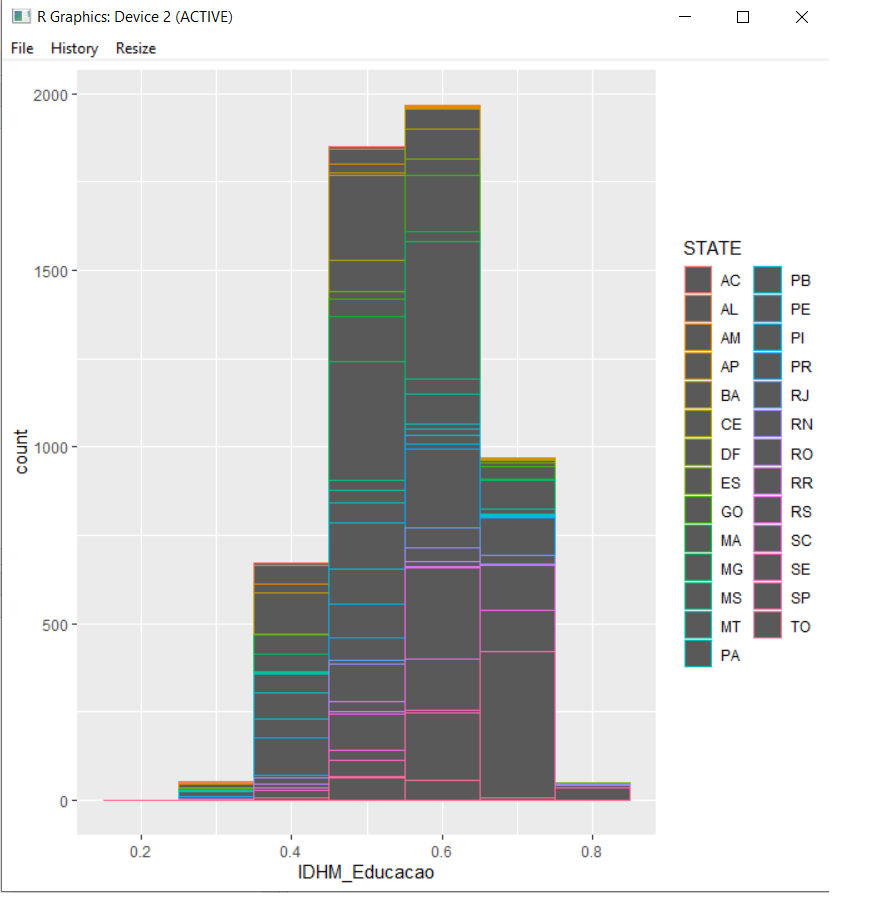
\includegraphics[scale=0.5]{chapter-03-case-01-img-04}
  \legend{Fonte: O autor}
\end{figure}

Dado os gráficos acima, foram realizados cálculos para conseguir realizar conclusões mais assertivas. Foram realizados cálculos de média simples e desvio padrão (desigualdade entre os dados, sendo 0 mais próximo da igualdade e 1 mais próximo da desigualdade).

Calculando a média de cada critério do IDH, foi constatado que a renda teve a nota 0.65, a longevidade teve a nota 0.80 e a educação teve a nota 0.55.

Agora calculando o desvio padrão de cada critério do IDH, foi constatado que a renda teve a nota 0.08, a longevidade teve a nota 0.04 e a educação teve a nota 0.09.

